\documentclass{llncs}



\newcommand\maroua[1]{\textcolor{red}{#1}}

\usepackage[modulo]{lineno}
\linenumbers
%\pagestyle{plain}

\usepackage{paralist}
\usepackage[colorinlistoftodos,prependcaption]{todonotes}
\usepackage{hyperref}
\usepackage{caption}
\graphicspath{{figures/}}

\usepackage [T1]{fontenc}
\usepackage[style=alphabetic, maxnames=99]{biblatex}
\addbibresource{references.bib}

\usepackage{enumitem}      % adjust spacing in enums

\newcommand\var[1]{\ensuremath{\mathtt{#1}}}
\newcommand{\keyword}[1]{\textsf{#1}}


\setcounter{biburllcpenalty}{7000}
\setcounter{biburlucpenalty}{8000}

\begin{document}
%\setcounter{page}{1}
\pagenumbering{arabic}

\title{Safe Dynamic Memory Management in Ada and SPARK}

\maketitle
\begin{abstract}
Handling memory in a correct and efficient way is a step toward safer, less complex, and higher performing software and software-intensive systems. However, languages used for critical software development such as Ada, which supports formal verification with its SPARK subset, face challenges regarding any use of pointers due to potential pointer aliasing. In this work, we introduce an extension to the Ada language, and to its SPARK subset, to provide pointer types (``access types'' in Ada) that provide provably safe, automatic storage management without any asynchronous garbage collection, and without explicit deallocation by the user. Because the mechanism for these safe pointers relies on a strict control of aliasing, they can be used in the SPARK subset for formal verification, including both information flow analysis and proof of safety and correctness properties. In this paper, we present this proposal (which has been submitted for inclusion in the next version of Ada), as explain
how we would be able to incorporate these pointers into formal analyses.
\end{abstract}

%\category{D - Software}{D.3 Programming Languages}{D.3.4 Processors - Compilers}


\keywords

Compilation, Safe Pointers, Formal Verification, Memory Management


\section{Introduction}

Standard Ada supports safe use of pointers (``access types'' in Ada) via strong type checking, but safety is guaranteed only for programs where there are no explicit deallocations of pointed-to objects -- explicit deallocation is considered ``unchecked'' programming in Ada, meaning that the programmer is responsible for ensuring that the deallocation is not performed prematurely. Ada can provide automatic reclamation of the entire memory pool associated with a particular pointer type when the pointer type goes out of scope, but it does not automatically reclaim storage prior to that point. It is possible for a user to implement abstract data types that do some amount of automatic deallocation at the object level, but this requires additional programming, and typically has certain limitations. As part of its strong type checking, Ada also prevents dangling references to objects on the stack or the heap, by providing automatic compile-time checking of ``accessibility'' levels, which reflect the lifetimes of stack and heap objects.  Conversions between pointer types are restricted to ensure pointers never outlive the objects they designate. Values of a pointer type are by default initialized to null to prevent use of uninitialized pointers, and run-time checks verify that a null pointer is never dereferenced.


SPARK is a subset of the Ada programming language, targeted at the most safety- and security-critical applications. SPARK starts with the basic Ada features oriented toward building reliable and long-lived software, then adds restrictions that ensure that the behavior of a SPARK program is unambiguously defined, and simple enough that formal verification tools can perform an automatic assessment of conformance between a program specification and its implementation. The SPARK language and toolset for formal verification have been applied over many years to on-board aircraft systems,
air traffic control systems, cryptographic systems, and rail systems \cite{ONeill2012, McCormick2015}.

As a consequence of our focus in SPARK on proof automation and usability, we have forbidden the use in SPARK of programming language features that either prevent automatic proof, or make it possible only at the expense of extensive user effort in annotating the program. The lack of support for pointers in SPARK is the main example of this choice. On the one hand, SPARK supports many Ada features that can make up for the lack of pointers: by-reference parameter passing, the ability to specify the address of objects, and the support for arrays as first-class objects. On the other hand, pointers are sometimes desirable, which forces one to exclude from formal SPARK analysis the parts of a program that make use of pointers. While there are idioms that facilitate this isolation of pointers in non-SPARK parts of a program~\cite{AdaCoreThalesSPARK}, it is highly desirable to provide some level of support for pointers in SPARK.

In this work, we present the first step for the inclusion of a variety of pointers that support safe memory management in Ada, in a way that these pointers can be included in SPARK. As our main contribution, we show that it is possible to adapt the ideas underlying the safe support for pointers in permission-based languages like Rust \cite{Balasubramanian17} or ParaSail \cite{Taft11}, to safely restrict the use of pointers in more traditional imperative languages like Ada. In section~\ref{sec:ownership-Ada}, we describe the rationale for the rules that we propose to include in the next version of Ada, which takes into account specificities of Ada like by-copy/by-reference parameter passing and exception handling. In section~\ref{sec:ownership-SPARK}, we outline how these rules would make it possible to formally verify programs with pointers with the SPARK toolset. We finally present related works and conclude.

\section{A Proposal for Ownership Types in Ada}
\label{sec:ownership-Ada}

Pointers (access types) are essential to many complex Ada data structures, but they also have some downsides, and can create various kinds of safety and security problems.
When attempting to prove properties about a program, particularly programs with multiple threads of control, the enemy is often the unknown ``aliasing'' of names introduced by
access types and certain uses of (potentially) by-reference parameters. We say that two names may alias if they have the possibility to refer to overlapping memory regions.
By \textit{unknown} aliasing of names, we mean the situation where two distinct names might refer to the same object, without the compiler being aware of that.  A rename introduces
an alias, but not an ``unknown alias,'' because the compiler is fully aware of such an alias, and hence is not something we are worrying about here. However, if a global
variable is passed by reference as a parameter to a subprogram that also has visibility on the same global, the by-reference parameter and the global are now aliases within
the subprogram, and the compiler generating code for the subprogram has no way of knowing that, hence they are ``unknown aliases.''  One approach is to always assume the worst,
but that makes analyses much harder, and in some cases infeasible. Access types also introduce unknown aliasing, and in most cases, an analysis tool will not be
sure whether the aliases exist, and will again have to make worst-case assumptions, which again may make any interesting proof infeasible.


The question that emerges in this context is: can we create a subset of access-type functionality that supports the creation of interesting data structures without bringing along
the various problems associated with unknown aliasing? The notion of pointer ``ownership'' has emerged as one way to ``tame'' pointer problems, while preserving flexibility \cite{POM}.  The goal is to allow a pattern of use
of pointers that avoids dangling references as well as storage leaks, by providing safe, immediate, automatic reclamation of storage rather than relying on unchecked deallocation,
while also not having to fall back on the time and space vagaries of garbage collection.  As a side benefit, we can also get safer use of pointers in the context of parallelism.
\todo[inline]{Several times it is stated that the proposed pointers will enhance parallel computing. I would have liked to see an example for this claim}
\todo[inline]{I would like the authors to comment on the implications of concurrent tasking with this proposed model}
We propose the use of pointer ownership (as well as some additional rules, detailed in \cite{AI2018}, preventing ``aliasing'' between parameters, and between parameters and global variables) to provide safe,
automatic, parallelism-friendly heap storage management while allowing the flexible construction of pointer-based data structures, such as trees, linked lists, hash tables, etc.

Although we took inspiration from Rust and ParaSail to produce this proposal, it is also different in many ways, due to the different objectives pursued in Ada and SPARK. Firstly,
this proposal is designed to work well with existing features of Ada such as by-copy/by-reference parameter passing and exception handling: raising an exception should not lead to
memory leaks, and upon handling of a raised exception, visible objects should not be left in an inconsistent state. Secondly, this proposal relies on the existing mechanisms in Ada
for preventing access to uninitialized pointers and out-of-scope memory: uninitialized and freed pointers should be set to null so that attempts at dereferencing such pointers result in a run-time error.


\subsection{Ownership Types}
\label{sec:ownership}

In this section, we describe the \textit{Ownership} aspect, a Boolean value which can be specified True for an Ada access type, with the effect that the compiler enforces an additional set of rules to ensure that there can be at most one writable access path to the data
\textit{designated} (i.e. pointed to) by an object of such an access type, or alternatively one or more read-only access paths via such access objects, but never both concurrently. This is known as
the Concurrent-Read-Exclusive-Write (CREW) access policy \cite{CREW}. The CREW policy prevents multiple access via different objects to the same memory area whenever one
of those access objects is modifying that area.


In addition to access types, Ownership can also be specified True for composite types, allowing for a record, an array, or even a private type with potentially multiple components that are access objects with Ownership True.  Any object of a type with Ownership True is called an \textit{ownership} object.
In addition, we use the more general term \textit{managed object} to refer to an ownership object or any object that is reachable by following ownership access objects.
Here is the overall taxonomy:

\begin{compactitem}
\item \textit{Ownership} objects: objects of a type with Ownership aspect True, including:
    \begin{compactitem}
\item \textit{Owning access} objects: access-to-variable objects with Ownership aspect True;
\item \textit{Observing access} objects: access-to-constant objects with Ownership aspect True;
\item \textit{Composite ownership} objects: records and arrays with Ownership aspect True;
    \end{compactitem}
\item Other \textit{managed} objects: non-ownership objects that are pointed to by an owning or observing access object.
\end{compactitem}


In the remainder, we presume that all objects in the code samples that we will present are managed objects; we refer the reader to \cite{AI2018} for further details on
the Ownership aspect specification, and specific rules that apply to non-ownership managed objects. Note also that some of the Ownership rules will be expressed in terms
of ``names'' rather than ``objects,'' since objects do not really exist at compile-time, when these rules are intended to be enforced.


In the next section, we will focus on owning access objects and observing access objects, which in Ada when passed as a parameter are passed by copy, before we
consider the situation of composite ownership objects, for which we require pass-by-reference.  As it turns out, when worrying about ownership and limiting the number of ways you can reach an object, whether something is passed by copy or by reference as part of calling another subprogram can make a difference, particularly in the context of propagating and handling exceptions.


\subsection{Ownership for Access Objects}
\label{subsec:ownershipAccess}

To ensure safe memory management, the basic rule is that at most one object of an access type that gives update access may be used to refer to a designated object at any time.  There might be multiple access objects that designate the same object (or some part of it) at any given time, but at most one of them may be used for updating that object.  And only when there are no updaters available, we allow one or more access objects that provide read-only access.


The manipulation of ownership access objects in the program is limited to the following three specific kinds of operations:

\begin{compactitem}
  \item \textit{Moving}: An assignment operation that leads to moving the value of one access object into another, leaving behind a null;
  \item \textit{Borrowing}: The declaration of a short-term read-write reference by copying an existing access object, borrowing its value for the lifetime of the \textit{borrower}.
  \item \textit{Observing}: The declaration of a short-term object that gives read-only access, by copying an existing access object, observing the object(s) reachable from it for the lifetime of the \textit{observer}.
\end{compactitem}

Given an access object, it should have one of these three possible states at any point in its scope:

\begin{compactitem}
  \item \textit {Unrestricted}: the object may be dereferenced and used to read or update the designated object;
  \item \textit {Observed}: the object may be used for read-only access to all or part of the designated object, or part of some object directly or indirectly reachable via a chain of owning access objects from the designated object;
  \item \textit {Borrowed}: the object's ownership has been temporarily transferred to another object,  and while in such a state the original access object is not usable for reading or updating the designated object (nor for any other purpose).
\end{compactitem}


\subsubsection{Moving Access Values}
\label{sec:moving}

The main idea of the \textit{move} operation is a complete transfer of the ownership from the right hand side to the left hand side in an assignment operation, where both left- and right-hand-side objects are owning access variables in the unrestricted state.
After the assignment, the right-hand side gets set to null, and the newly assigned object becomes the (unrestricted) owner. By setting the original access object to null, any name that starts with a dereference of
that original access object is effectively ``destroyed,'' and we ensure that even if an exception is raised before we explicitly assign a new value to the right-hand side, upon handling the exception, there is no danger it will
be able to dereference the old value of the right-hand side.  Being allowed to use the old value to reach the designated object would, at a minimum, violate our CREW policy, and would be much worse if the designated object had been deallocated after the move, but prior to the exception being raised.


In addition to setting the right-hand side to null, a move also finalizes and deallocates the object, if any, designated by the
left-hand side prior to the assignment.  This automatic deallocation means memory is reclaimed as soon as it is
no longer accessible, thereby preventing memory leaks, without the need for an asynchronous garbage collector.
This is safe to do, because a move requires the left-hand side to be in the \textit{unrestricted} state, meaning that
the left-hand side is the only access object pointing to the object about to be deallocated.


In addition to considering certain assignment statements to be \textit{moves}, we also consider the assignment
operations inherent in passing an \keyword{out} or \keyword{in out} parameter to be moves, as well
as the assignment inherent in returning a value from a function.
Assignments that are part of updating a subcomponent of a composite object are also considered moves, but
we consider those in a later section focused on composite types (see below).


Figure \ref{fig:move_ex1} illustrates an example of ``move'' operations. Objects \var{X} and \var{Y} are access-to-variables objects of the named type \var{Int\_Ptr}. At a \var{Swap} procedure call site,
the actual parameter \var{X}, which is required to be in the unrestricted state, is \textit{copied in} to the formal \var{X\_Param}. The \textit{ownership} of \var{X.all} (\var{X.all} is Ada's notation for dereferencing X -- \var{X.all} denotes the object \textit{designated} by X) is similarly moved from \var{X} to \var{X\_Param}.
That requires setting \var{X} to null until the subprogram returns (to ensure safety in the presence of an exception), at which point the final value of \var{X\_Param} is \textit{copied back} to \var{X}.
Variable \var{X} then reasserts its ownership over \var{X.all}. Similar state transitions apply for \var{Y} and \var{Y\_Param}.  At lines $\ell_4$, $\ell_6$, and $\ell_7$,
we have additional move operations, which consist of moving, respectively, the objects \var{X\_Param}, \var{Y\_Param}, and \var{Tmp}. Thanks to our move-related rules, even such a straightforward
implementation of the Swap procedure for access types is nevertheless guaranteed to be alias safe while \var{Swap} is executing, both from the \textit{caller} perspective and from \textit{inside} \var{Swap} itself, since the ownership is transferred
as part of each access-to-variable object copy.

\begin{figure}[htb!]
\centering
   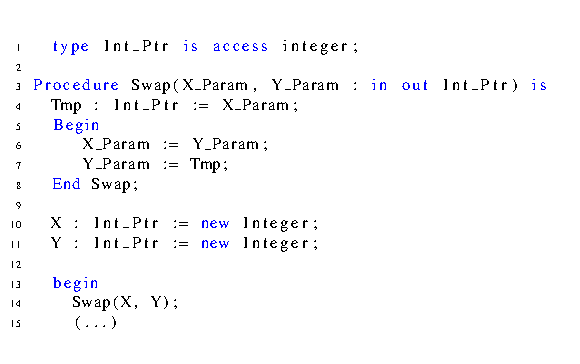
\includegraphics[]{move_ex1}
   \caption{Example of moving the ownership of an object.}
   \label{fig:move_ex1}
\end{figure}

\subsubsection{Borrowing Access Values}
\label{sec:borrowing}

We say that an access value has been ``borrowed'' if that value has been copied into a short-lived (owning) access-to-variable  object.
The key feature of a borrowing operation is a \textit{temporary} transfer of the ownership of the said borrowed object until the end of the scope of the borrower.
We want the original access value to still designate the same object until the borrower goes away. As a result, while an access object
is in the borrowed state, its value may not be changed; furthermore, to preserve our CREW policy, we want to be sure it is not used or copied again until the current borrower goes away, so in fact when in the borrowed state, the original access object is completely ``dead''; it cannot
be read nor be the target of an assignment. Furthermore, borrowing applies recursively down the tree rooted at the original access object, meaning that at the point where a name is borrowed,
every name with that name as a prefix, is similarly borrowed.


The assignment operations that are considered borrowing are those that \textit{initialize} a stand-alone object of an \textit{anonymous} access-to-variable type, or a \keyword{constant} or an \keyword{in} parameter of a (named or anonymous) access-to-variable
type.  We also consider as borrowing the passing of an object of a composite ownership type
as a parameter of mode \keyword{out} or \keyword{in out} -- we will expand on this in Section \ref{subsec:ownershipComposite} below. For now, let us consider the
code snippet of Figure \ref{fig:borrow_ex1} as a simple example of borrowing. \var{X} and \var{Y} are both access-to-variable objects. We want to swap the objects \textit{designated} by the two
pointers (their ``contents'') using the \var{Swap\_Contents} procedure. To that end, we declare \var{X\_Param} and \var{Y\_Param} as formal parameters of mode \keyword{in}. Objects \var{X} and \var{Y} become borrowed
in the caller, and inside \var{Swap\_Contents} \var{X\_Param} and \var{Y\_Param} are the borrowers, in the unrestricted state. This state allows reading and updating via these formal parameters, which makes swapping
the value of their designated objects safely possible. Note that we allow an \keyword{in} parameter or a stand-alone constant of an owning access type to provide read/write access to its designated object to accommodate existing Ada practice in the use of such ``constant'' access-to-variable values to nevertheless update their designated objects.

\begin{figure}[htb!]
\centering
   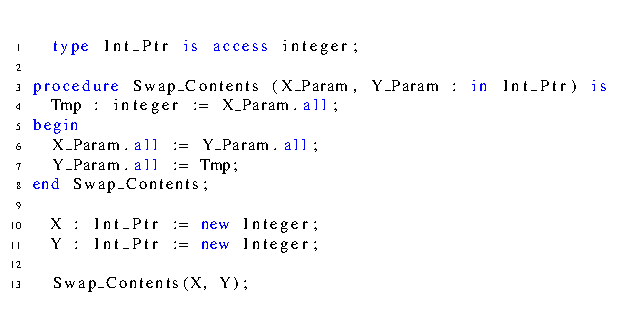
\includegraphics[]{borrow_ex1}
   \caption{Example of borrowing via \keyword{in} parameters.}
   \label{fig:borrow_ex1}
\end{figure}


\subsubsection{Observing Access Values}
\label{sec:observing}

We say an access-to-variable object is ``observed'' when its value has been copied into an ``observer,'' and both the original
access object and the copy, starting at that point, can only be used for gaining read access to the designated object.
The original object remains in the observed state until the end of the scope of the observer. While being observed, neither the observed object nor the observer is allowed to be moved or
borrowed. The original access object must not be used as the target of an assignment since we want the observed object to continue
to designate the same object as long as any observers exist.  As with borrowing, observing applies recursively down the tree rooted at the original access object, meaning that at the point where a name is observed,
every name with that name as a prefix, is similarly observed.


We consider as observing the assignment operations used to \textit{initialize} stand-alone objects of an anonymous access-to-\textit{constant} type, as well as \keyword{in} parameters of such a type.
In the code snippet of Figure \ref{fig:observe_exp}, \var{X\_Param} and \var{Y\_Param} are access-to-constant objects of an anonymous type. Since the assignment of the value of \var{X} to \var{X\_Param}
as well as to \var{Y\_Param} are part of the initialization of the target objects, this initiates the observing, and while \var{X\_Param} and \var{Y\_Param} exist they provide read-only access. Note that
this allows us to call the function \var{Sum} using \var{X} as a first and second parameter -- upon the first occurrence of \var{X} it enters the observed state, but we can still observe it further.
%\maroua{Note that while the call to \var{Sum} is in progress, variale \var{X} is observed and therefore cannot be modified by any other task that has visibility on it. (to answer the comment below)}

\begin{figure}[htb!]
\centering
   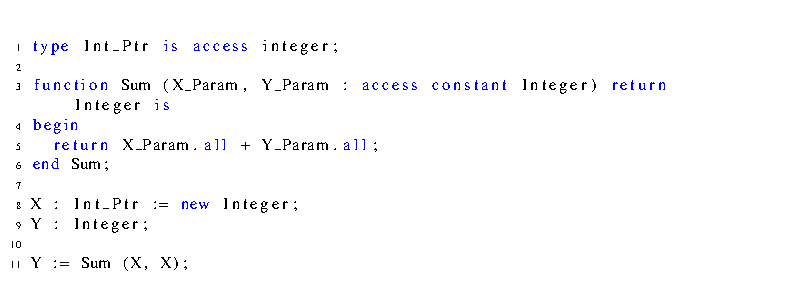
\includegraphics[]{observe_ex1}
   \caption{Example of observing via access-to-constant parameters.}
   \label{fig:observe_exp}
\end{figure}

\todo[inline]{For instance, in Figure 3, how can you prove that another task that has visibility over variable X is not concurrently modifying the object pointed to by X while the call to Sum is in progress?}


\subsubsection{Preventing Read-Write Aliasing}
\label{sec:noaliasing}

We have seen that the observing rules allow multiple access objects to observe the same designated object. In the scope of these objects, the original object is in the observed state, meaning that its designated object
cannot be written, so there is no read-write aliasing problem here.


We have seen that after borrowing an object, its name allows neither reading nor updating until the borrowing ends. For example, this prevents a call to \var{Swap\_Contents (X, X)},
as borrowing X via parameter \var{X\_Param} makes it illegal to borrow it again via parameter \var{Y\_Param}. The actual order of evaluation does not matter here, as any other order would also be illegal.


We have also seen that after moving an object, its value is set to null, which prevents accessing the designated object again through the original name.
That rule by itself does not prevent a call to \var{Swap(X, X)}, but moving \var{X} into parameter \var{X\_Param} makes \var{X} null, so that if it is then moved into parameter \var{Y\_Param}, the value null will be passed.   As it turns out, passing the same object twice in the same call, as an \keyword{out} or \keyword{in out} parameter, is already illegal in current Ada.
Even without this Ada rule, there is no danger of read-write aliasing inside \var{Swap}. However, if the code were legal, the actual order of evaluation would matter for the functional behavior, as another order would make \var{X\_Param} null
instead. Likewise, on return from the procedure call, if the call were legal, moving back parameter values to \var{X} could happen in two different orders.
While simple cases of parameter aliasing like \var{Swap(X,X)} are already illegal in current Ada, more complex cases that involve, for example, dynamic array indexing are neither
prevented by current Ada rules nor by the rules for moving presented previously. Therefore, as part of the proposed
extension to Ada, an additional restriction \var{No\_Parameter\_Aliasing} has been proposed,
which will prevent the more complex cases as well. We refer the reader to \cite{AI2018} for further details on the \var{No\_Parameter\_Aliasing} restriction.


\subsection{Extension to Composite Types}
\label{subsec:ownershipComposite}

The rules presented previously for access objects are extended in natural ways to composite ownership objects (records or arrays with owning access objects as subcomponents) to enforce the Concurrent-Reads-Exclusive-Write principle.

\subsubsection{Moving Composite Values}
\label{subsubsec:movingComposite}

As with access objects, the main idea of the composite move operation is a complete transfer of the ownership from the right hand side composite object to the left hand
side object as part of an assignment operation. And as with access objects, a moved composite object should be in the unrestricted state before the assignment. The rules that apply for moving an
access object are applied here to each access subcomponent of the composite type: access subcomponents of the moved objects are set to null after being copied, and to avoid memory leaks, if the
prior value of the subcomponent in the target composite object is different from the new value, the object designated by this prior value is finalized and its storage is deallocated.

As before, we consider as a move each assignment operation for a composite ownership type where the target is a variable (or the object returned by a function), but this time we do not
consider passing of \keyword{out} or \keyword{in out} parameters to be moves, because for composite ownership objects, parameters are passed by reference and no true copying is occurring. Composite parameter passing is described further below.

In the code snippet of Figure~\ref{fig:movingComposite}, \var{Rec} is a record with components of an owning access type. The move operation occurs at line $\ell_{9}$ where \var{R} is moved
to \var{S}, which involves moving \var{R.X} into \var{S.X} and moving \var{R.Y} into \var{S.Y}. As a result, the objects originally designated by
\var{S.X} and \var{S.Y} are deallocated and \var{R.X} and \var{R.Y} end up null after the assignment.


\begin{figure}[htb!]
\centering
   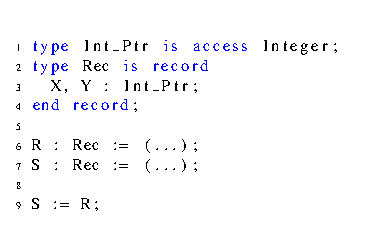
\includegraphics[]{movingComposite}
   \caption{Example of moving a composite object.}
   \label{fig:movingComposite}
\end{figure}

\subsubsection{Borrowing Composite Values}
\label{subsubsec:borrowComposite}

Borrowing composite ownership objects occurs when passing such an object as an \keyword{out} or \keyword{in out} parameter, consistent with
these composite ownership objects being passed by reference. Note how this differs from \keyword{out} or \keyword{in out} parameters of an access type, which are passed by copy,
and are thus considered as being \textit{moved} as part of parameter passing. Ada normally allows composite objects to be passed either by copy or by reference, but for ownership composite types, we require they always be passed by reference, to avoid having two different sets of rules for composite objects which would depend on whether the type is passed by copy or by reference.

In the code snippet of Figure~\ref{fig:borrowingComposite}, procedure \var{Swap\_Rec} has an \keyword{in out} formal parameter \var{R} of a record type. At the point of
call to \var{Swap\_Rec}, the actual parameter name \var{R1} becomes borrowed until returning from \var{Swap\_Rec}, with the borrower being the formal parameter name \var{R}.  Inside \var{Swap\_Rec}, the formal parameter \var{R} is initially
in the unrestricted state, hence its components \var{R.X} and \var{R.Y} can be successively moved in and out through the call to \var{Swap}, and then borrowed through the call to \var{Swap\_Contents}.
Note that subcomponents of a composite type can be individually moved and borrowed, without impacting the state of other non-overlapping subcomponents of the same composite object.
We refer the reader to \cite{AI2018} for further details.

\begin{figure}[htb!]
\centering
   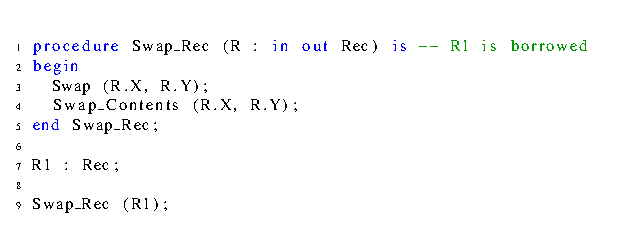
\includegraphics[]{borrowingComposite}
   \caption{Example of borrowing via a composite \keyword{in out} parameter.}
   \label{fig:borrowingComposite}
\end{figure}


\subsubsection{Observing Composite Values}
\label{subsubsec:extendingBorrowing}

Observing composite ownership objects occurs when passing such an object as an \keyword{in} parameter, or initializing a constant stand-alone object of such a type.

In the code snippet of Figure~\ref{fig:observingComposite}, procedure \var{Sum\_Rec} has an \keyword{in} formal parameter \var{R} of a record type.
At the point of call to \var{Sum\_Rec}, the actual parameter name \var{R1} becomes observed, with the formal parameter \var{R} as the observer, until returning from \var{Sum\_Rec}. Inside \var{Sum\_Rec},
the formal parameter \var{R} is initially in an observed state, hence its components \var{R.X} and \var{R.Y} can only be read (observed) through the call to \var{Sum}.


\begin{figure}[htb!]
\centering
  \captionsetup{justification=centering,margin=0.6cm}
   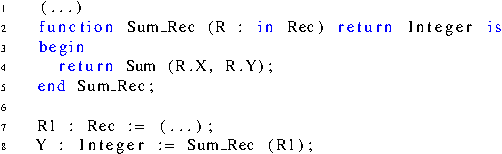
\includegraphics[]{observingComposite}
   \caption{Example of read only access to an object of a composite type.}
   \label{fig:observingComposite}
\end{figure}


\subsubsection{Traversing Data Structures with Local Variables}

In the rules for borrowing access values (Section~\ref{sec:borrowing}), we said that initializing a stand-alone object of an anonymous access-to-variable type corresponds to
\textit{borrowing} the access object being copied. Similarly, in the rules for observing access values (Section~\ref{sec:observing}), we said that initializing a stand-alone object of an
anonymous access-to-constant type corresponds to \textit{observing} the object being copied. Without these special cases, such initializations might be treated as moves, which would not allow for a non-destructive
traversal of a recursive data structure, since every assignment to such a ``handle'' would
deallocate its prior designated object and set to null the object that was moved.  Hence, these objects of an anonymous access type acts as a kind of short-term ``handle'' on the tree of objects rooted at the original access object.

We also allow certain kinds of updates to such ``handles,'' in order to allow traversing the data structure by changing where the handle points.
In the borrowing case (for an access-to-\textit{variable} object), we allow the borrower to be updated to point to an object within the tree rooted at the prior value of the borrower; this is not considered a new borrowing action, as the existing borrower remains the only object providing any read or write access to the subtree rooted at its original value.
By limiting the initial borrowing to the initialization of a new stand-alone object, we ensure that borrowing lasts only as long as the lifetime of the ``handle.''  If we allowed any given assignment statement to initiate a new borrowing action, tracking when such borrowing would end might require complex data-flow analysis, potentially across conditional and iterative paths in the program.  Somewhat less stringent restrictions are applied when updating an observer -- the observer may be updated to point to an already observed object with a compatible scope. Again, doing otherwise might require complex data-flow analysis to determine the extent of the observing action.

In the code snippet of Figure~\ref{fig:maxTree}, local variable \var{Walker} is a stand-alone object of an anonymous access-to-\textit{constant} type, which allows traversing the input binary
search tree, so as to find the maximal value (obtained by searching for the rightmost leaf of the tree). After initializing \var{Walker} with the value of parameter \var{T},
\var{T} becomes observed, and \var{Walker} starts in the observed state (thus preventing updates to \var{T.all} through \var{Walker}). The data structure traversal is performed by the instruction
of line $\ell_{16}$.

\begin{figure}[htb!]
\centering
  \captionsetup{justification=centering,margin=0.6cm}
   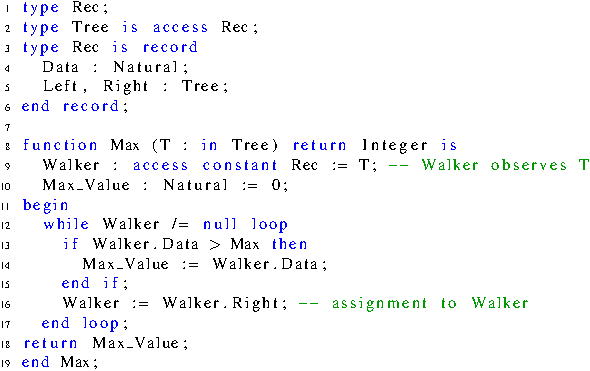
\includegraphics[]{maxTree}
   \caption{Example of traversing a data structure with read-only access: Max on a Binary Search Tree.}
   \label{fig:maxTree}
\end{figure}

In the code snippet of Figure~\ref{fig:treeInsert}, local variable \var{Walker} is a stand-alone object of an anonymous access-to-\textit{variable} type, which allows traversing the input binary
search tree to insert the input value \var{V} at the correct leaf position (obtained by searching for the branch where this value would be stored, if it were already present).
After initializing \var{Walker} with a copy of the value of parameter \var{T}, \var{T} becomes borrowed, and \var{Walker} starts its life in the unrestricted state (thus allowing updates via \var{Walker} to the tree pointed to by \var{T}).
The data structure traversal is performed by the instruction of line $\ell_8$ and $\ell_{15}$. Insertion in the tree is performed at lines
$\ell_{10}$ and $\ell_{17}$.


\begin{figure}[htb!]
\centering
  \captionsetup{justification=centering,margin=0.6cm}
   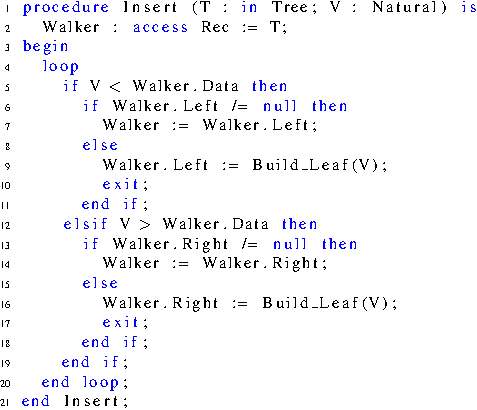
\includegraphics[]{treeInsert}
   \caption{Example of traversing a data structure with read and  update access: Insert into a Binary Search Tree. \var{Build\_Leaf(V)} creates a node with \var{Data} = \var{V}, and \var{Left}, and \var{Right} components both null.}
   \label{fig:treeInsert}
\end{figure}

%\todo[inline]{I would have liked to see how a node is deleted from such a tree}

\section{Formal Verification with Ownership Types in SPARK}
\label{sec:ownership-SPARK}

The existing SPARK restrictions imposed on its current subset of Ada ensure that an assignment to one variable cannot change the value of some other visible variable. This property is essential to allow sound modular static analysis,
where each subprogram can be analyzed independently while detecting all possible violations of the kinds targeted by the analysis.

This is currently enforced by forbidding all use of access types in SPARK, and by restricting aliasing between parameters and global variables so that only
benign aliasing is permitted (i.e. aliasing that does not cause interference).  The aliasing restrictions are as follows:


\begin{compactitem}
  \item Two output parameters should never be aliased.
  \item An input and an output parameters should not be aliased, unless the input parameter is always passed by copy.
  \item An output parameter should never be aliased with a global variable referenced by the subprogram.
  \item An input parameter should not be aliased with a global variable referenced by the subprogram, unless the input parameter is always passed by copy.
\end{compactitem}

\smallskip
To understand why aliasing matters in SPARK, consider procedure \var{Add\_One} in Figure~\ref{fig:spark_ex1}. If \var{X\_Param} and \var{Y\_Param}
are not aliased, then the result of calling \var{Add\_One} on actual parameters \var{X} and \var{Y} will increase their contents by one. If \var{X} and \var{Y} are aliased, then calling
\var{Add\_One} on \var{X} and \var{Y} will increment the underlying content by two.


\begin{figure}[htb!]
\centering
  \captionsetup{justification=centering,margin=0.6cm}
   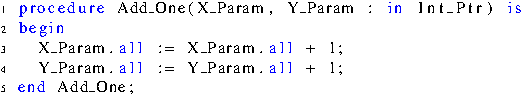
\includegraphics[]{spark_ex1}
   \caption{A simple procedure where aliasing would create problems in SPARK.}
   \label{fig:spark_ex1}
\end{figure}

If SPARK ignored aliasing, it would conclude that procedure \var{Add\_One} always increments by exactly one the content of each of its parameters \var{X\_Param} and \var{Y\_Param}.
In particular, it could prove the following postcondition on the procedure.

\begin{figure}[htb!]
\centering
  \captionsetup{justification=centering,margin=0.6cm}
   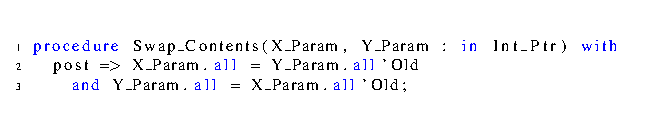
\includegraphics[]{spark_ex1_proof}
   \label{fig:spark_ex1_proof}
\end{figure}

Indeed, by presuming that the assignment to \var{X\_Param.all} on line $\ell_2$ does not influence the value of \var{Y\_Param.all}, proof would be able to
derive that the values \var{Y\_Param.all} has been incremented by 1. Similarly, flow analysis could derive wrong data dependencies if possible aliasing is not taken into account.

This wrong postcondition would in turn allow a proof that an incorrect assertion is satisfied in the code snippet of Figure \ref{fig:spark_ex1_exp}, while in fact it fails at run time:

\begin{figure}[htb!]
\centering
  \captionsetup{justification=centering,margin=0.6cm}
   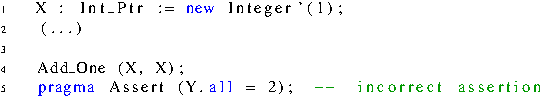
\includegraphics[]{spark_ex1_exp}
	\caption{Example of proof of an incorrect assertion due to the presence of aliasing in SPARK.}
   \label{fig:spark_ex1_exp}
\end{figure}

Thus, pointers cannot be treated like any other component in SPARK, in the presence of aliasing. But rules we have described for ownership objects precisely prevent
aliasing when one of the objects can be written. This is similar to the rules in SPARK for preventing aliasing between by-reference parameters, and this allows SPARK to treat such pointers
like other components.

In the case of \var{Add\_One}, this means that SPARK analysis will be able to conclude that the postcondition above is satisfied by the implementation of \var{Add\_One}.
But calls to \var{Add\_One(X,X)} will be rejected both by compilation and analysis.


\section{Related Work}

Permission-based programming languages generalize the issue of avoiding harmful aliasing to the more general problem of preventing harmful sharing of resources
(memory, but also network connections, files, etc.). C-like languages are mostly based on pointers and often sacrifice safety for performance purposes.
To overcome safety shortcoming and manage the storage of a pointer, C++ introduces the notion of \textit{unique pointers}. An object defined as a \var{unique\_ptr}
has the ability of taking ownership of an object. It becomes responsible for its deletion at some point. Although these rules help provide greater language safety, the unique
pointer concept is limited because it prohibits pointer arithmetic and copy assignments.

Separation logic~\cite{Reynolds02} is an extension of Hoare-Floyd logic that allows reasoning about pointers. In general, it is not well integrated with deductive
verification, and, in particular, is not supported by most SMT provers.


Dafny associates each object with its \emph{dynamic frame}, the set of pointers that it owns~\cite{Leino10}. This dynamic version of Ownership is
enforced by modeling the Ownership of pointers in logic, generating verification conditions to detect violations of the single-owner model, and proving
them using SMT provers. In Spec\#, Ownership is similarly enforced by proof, to detect violations of the so-called Boogie methodology~\cite{Boogie}.

The inspiration for much of our work springs from the system programming in Cyclone \cite{Grossman2002}, Rust \cite{Balasubramanian17}, and ParaSail \cite{Taft11}, which achieve absence of
harmful aliasing by enforcing an Ownership type system on the memory pointed to by objects. Rust and ParaSail are recent programming languages targeting system
programming, with a focus on memory safety for concurrent programs.
Rust and ParaSail also deal with the lifetime of allocated memory, enforcing
at the same time the lack of dangling pointer references.

The most closely related work to ours springs from Jaloyan \textit{et al.} \cite{Jaloyan18} anti-aliasing rules. In \cite{Jaloyan18}, access-to-variable objects
and composite objects with access subcomponent objects are considered as \textit{deep} variables and their ownership states are transferred in the same way when used to call subprograms.
Actual deep parameters are considered as borrowed and the durations of borrows are only limited to the duration of procedure calls.
It turns out that their rules do not allow traversing a linked data structure with read/write permission, or even traversing with read-only permission. In our work, the distinction between stand-alone access
objects and composite ones and moving or observing composite objects instead of borrowing them has allowed us to traverse a data structure, preserving the ability to modify objects reachable by following pointers.

In our work, we use a permission-based mechanism for detecting potentially harmful aliasing, in order to make the presence of pointers transparent for automated provers.
In addition, our approach does not require additional user annotations, which are required in some of the previously mentioned techniques.  We instead rely on the existing distinctions in Ada between \keyword{in} and \keyword{in out}parameters, and between access-to-variable and access-to-constant types. We thus achieve high automation
and usability, which was one of our goals in supporting pointers in SPARK.


\section{Conclusion}
We have presented an extension to the Ada language to provide pointer types (``access types'' in Ada) that provide provably safe, automatic
storage management without any asynchronous garbage collection, and without explicit deallocation by the user. Although we took inspiration
from Rust and ParaSail, the extension we propose is also different in many ways, in order to work well with existing features of Ada such
as by-copy/by-reference parameter passing and exception handling, and because we rely on the existing mechanisms in Ada for preventing access
to uninitialized pointers and freed memory.

This extension relies on the notion of ownership, where only one access object can provide read and update access to the designated object at any given time.
Ownership of a designated object can be \textit{moved} to another object through assignment, which deallocates the object previously designated
by the target of the assignment and leaves the source of the assignment null. Ownership can also be \textit{borrowed} giving a short-term borrower read-write access to the designated object; a borrower
can be either a parameter or a locally defined object. Finally, the value of a designated object can be \textit{observed} by multiple
read-only observers, with limited lifetimes. Collectively, these mechanisms enforce a principle of Concurrent-Reads-Exclusive-Write.

Because the mechanism for these safe pointers relies on a strict control of aliasing, they can be used in the SPARK subset for formal verification, which
includes both analysis of flows and proof of properties.

This proposal has been formalized as Ada Issue \cite{AI2018} for inclusion in the next version of Ada. We have also implemented a prototype of these permission rules in the GNAT/GCC
compiler for Ada developed at AdaCore. Our implementation successfully proves the safety of all programs presented in this article.

\paragraph{Acknowledgements.} We thank the anonymous reviewers for their
remarks, and Georges-Axel Jaloyan for his initial work on the design,
formalization and implementation of these ownership rules for Ada and SPARK.

\nolinenumbers
\printbibliography[title={References}]

\end{document}
\grid
